\documentclass[11pt,a4paper]{article}
\usepackage[left=2.5cm,right=2cm, bottom=2cm]{geometry}
\usepackage[utf8]{inputenc}
\usepackage{amsmath}
\usepackage{amsfonts}
\usepackage{amssymb}
\usepackage{amsfonts}
\usepackage{amsmath}
\usepackage{graphicx}
\usepackage{subfigure}
\usepackage{color}
\usepackage{abstract}
\usepackage{float}
\usepackage[toc,page]{appendix}
\usepackage{hyperref}
\usepackage{fancyhdr}
\usepackage{algorithm} 
\usepackage{algpseudocode} 
\usepackage{listings}
\usepackage{xcolor} % for setting colors
% set the default code style
\lstset{
	frame=tb, % draw a frame at the top and bottom of the code block
	tabsize=4, % tab space width
	showstringspaces=false, % don't mark spaces in strings
	numbers=left, % display line numbers on the left
	commentstyle=\color{green}, % comment color
	keywordstyle=\color{blue}, % keyword color
	stringstyle=\color{red} % string color
}

\pagestyle{fancy}
\fancyhf{}
\rhead{\today}
\lhead{\bfseries Alexander Leitner 01525882}
\rfoot{}



\begin{document}
\begin{center}
	\fontsize{24pt}{10pt}\selectfont
	\textsc{\textbf{Computational Science on Many-Core Architectures  Exercise 2}}
\end{center}
\section*{Example 1 Basic Cuda}
\subsection*{a)}
Seven different array length from $N = 10,100,1000,...10^8$ and its time for Malloc and Free.
\begin{figure}[H]
	\centering
	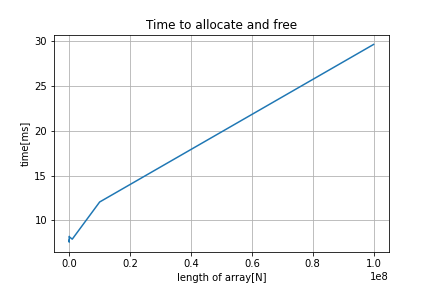
\includegraphics[width=0.70\textwidth]{Bilder/Time_to_allocate_and_free.png}
	\caption{5 turn}
\end{figure}
I run the code seven times and document the time results.
\begin{lstlisting}[language=C++, caption={code for a)}]
#include <stdio.h>
#include "timer.hpp"

int main(void)
{
	int N = 10;
	double *d_x;
	Timer timer;
	
	timer.reset();
	for (int i = 0;i < 100; i++)
	{
		cudaMalloc(&d_x, N*sizeof(double));
		cudaFree(d_x);
	}
	printf("Malloc_Free_Time: %g[ms] N = %d\n", (1000*timer.get())/100,N);
return EXIT_SUCCESS;
}
\end{lstlisting}
\newpage
\subsection*{b) Init by kernel}
\begin{lstlisting}[language=C++, caption={code for a)}]
#include <stdio.h>
#include "timer.hpp"

#include <vector>
#include <iostream>

__global__ void init_kernel(int N)
{
	double *x, *y;

	x = new double [N];
	y = new double [N];

	for (int i = 0; i < N; i++) 
	{
		x[i] = i;
		y[i] = N-i-1;
	}
}

int main(void)
{
	int N = 1000000;
	int M = 1;
	Timer timer;

	cudaDeviceSynchronize();
	timer.reset();

	init_kernel<<<(M+255)/256, 256>>>(N);
	cudaDeviceSynchronize();
	printf("Kernel_init_Time: %g[ms]\n", (1000*timer.get()));

	//Runtime 32.188[ms]
return EXIT_SUCCESS;
}
\end{lstlisting}
\newpage
\subsection*{b) Init by cudaMemcopy}
\begin{lstlisting}[language=C++, caption={code for a)}]
# include <stdio.h>
# include "timer.hpp"

int main (void)
{
	int N = 1000000;
	double *x, *y, *d_x, *d_y;
	Timer timer;

	x = new double[N];
	y = new double[N];

	for (int i = 0; i < N; i++)
	{
		x[i] = i;
		y[i] = N-i-1;
	}

	cudaDeviceSynchronize();
	timer.reset();

	cudaMalloc(&d_x, N*sizeof(double));
	cudaMalloc(&d_y, N*sizeof(double));

	cudaMemcpy(d_x, x, N*sizeof(double), cudaMemcpyHostToDevice);
	cudaMemcpy(d_y, y, N*sizeof(double), cudaMemcpyHostToDevice);

	cudaDeviceSynchronize();
	printf("Kernel_init_Time: %g[ms]\n", (1000*timer.get()));

	cudaFree(d_x);
	cudaFree(d_y);
	free(x);
	free(y);
return EXIT_SUCCESS;
//11.189[ms]
}
\end{lstlisting}
\newpage
\subsection*{b) Init by individual element cudaMemcopy}
\begin{lstlisting}[language=C++, caption={code for a)}]
# include <stdio.h>
# include "timer.hpp"

int main (void)
{
	int N = 1000;
	double *x, *y, *d_x, *d_y;
	Timer timer;

	x = new double[N];
	y = new double[N];

	for (int i = 0; i < N; i++)
	{
		x[i] = i;
		y[i] = N-i-1;
	}

	cudaDeviceSynchronize();
	timer.reset();

	cudaMalloc(&d_x, N*sizeof(double));
	cudaMalloc(&d_y, N*sizeof(double));
	for (int i = 0; i < N;i++)
	{
		cudaMemcpy(d_x+i, x+i, 1*sizeof(double), cudaMemcpyHostToDevice);
		cudaMemcpy(d_y+i, y+i, 1*sizeof(double), cudaMemcpyHostToDevice);
	}


	cudaDeviceSynchronize();
	printf("Kernel_init_Time: %g[ms]\n", (1000*timer.get()));

	cudaFree(d_x);
	cudaFree(d_y);
	free(x);
	free(y);

return EXIT_SUCCESS;

//41729.4[ms] N = 1000
}
\end{lstlisting}
For that point I only test the program with $N = 1000$ to reduce the time to ran the program. It is clear that this method is way slower than the other two.
\newpage
\subsection*{c) Kernel to sum up two vectors}
\begin{lstlisting}[language=C++, caption={code for a)}]
# include <stdio.h>
# include "timer.hpp"

__global__ void SumOfVectors(double *x, double *y, double *z, int N)
{
	int thread_id = blockIdx.x * blockDim.x + threadIdx.x;

	for (size_t i = thread_id; i < N; i += blockDim.x * gridDim.x)
	{
		z[i] = x[i] + y[i];
	}
}

int main (void)
{
	int N = 100;
	int s = 16
	double *x, *y, *z, *d_x, *d_y, *d_z;
	Timer timer;

	x = new double[N];
	y = new double[N];
	z = new double[N];

	for (int i = 0; i < N; i++)
	{
		x[i] = i;
		y[i] = N-i-1;
		z[i] = 0;
	}

	cudaMalloc(&d_x, N*sizeof(double));
	cudaMalloc(&d_y, N*sizeof(double));
	cudaMalloc(&d_z, N*sizeof(double));

	cudaMemcpy(d_x, x, N*sizeof(double), cudaMemcpyHostToDevice);
	cudaMemcpy(d_y, y, N*sizeof(double), cudaMemcpyHostToDevice);
	cudaMemcpy(d_z, z, N*sizeof(double), cudaMemcpyHostToDevice);

	cudaDeviceSynchronize();
	timer.reset();

	SumOfVectors<<<s, s>>>(d_x, d_y, d_z, N);
	cudaDeviceSynchronize();

	cudaMemcpy(z, d_z, N*sizeof(double), cudaMemcpyDeviceToHost);

	printf("SumTime: %g[ms]\n", (1000*timer.get()));
	printf("FirstEntrieOfSumVec: %f\n",z[N]);


	cudaFree(d_x);
	cudaFree(d_y);
	cudaFree(d_z);
	free(x);
	free(y);
	free(z);
return EXIT_SUCCESS;
}
\end{lstlisting}
\subsection*{d) Kernel to sum up two vectors with different N}
\begin{lstlisting}[language=C++, caption={code for a)}]
# include <stdio.h>
# include "timer.hpp"

__global__ void SumOfVectors(double *x, double *y, double *z, int N)
{
	int thread_id = blockIdx.x * blockDim.x + threadIdx.x;

	for (size_t i = thread_id; i < N; i += blockDim.x * gridDim.x)
	{
	z[i] = x[i] + y[i];
	}
}

int main (void)
{
	int N = 100;
	int anz = 100;
	double *x, *y, *z, *d_x, *d_y, *d_z;
	Timer timer;

	x = new double[N];
	y = new double[N];
	z = new double[N];

	for (int i = 0; i < N; i++)
	{
		x[i] = i;
		y[i] = N-i-1;
		z[i] = 0;
	}

	cudaMalloc(&d_x, N*sizeof(double));
	cudaMalloc(&d_y, N*sizeof(double));
	cudaMalloc(&d_z, N*sizeof(double));

	cudaMemcpy(d_x, x, N*sizeof(double), cudaMemcpyHostToDevice);
	cudaMemcpy(d_y, y, N*sizeof(double), cudaMemcpyHostToDevice);
	cudaMemcpy(d_z, z, N*sizeof(double), cudaMemcpyHostToDevice);

	cudaDeviceSynchronize();
	timer.reset();

	for (int i = 0; i < anz; i++)
	{
		SumOfVectors<<<(N + 255)/256, 256>>>(d_x, d_y, d_z, N);
		cudaDeviceSynchronize();
	}
	cudaDeviceSynchronize();
	printf("MidSumTime: %g[ms]\n", (1000*timer.get())/anz);
	cudaMemcpy(z, d_z, N*sizeof(double), cudaMemcpyDeviceToHost);

	cudaFree(d_x);
	cudaFree(d_y);
	cudaFree(d_z);
	free(x);
	free(y);
	free(z);

return EXIT_SUCCESS;
}
\end{lstlisting}
\begin{figure}[H]
	\centering
	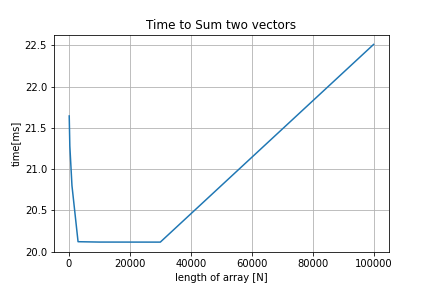
\includegraphics[width=0.70\textwidth]{Bilder/Time_to_Sum.png}
	\caption{5 turn}
\end{figure}
The time differenz between small number of $N$ and a large number of $N$ is very small $ 2.5$[ms]. I would expact a larger timedifferenz.
\newpage
\subsection*{e) Different size of blocks and grid}
\begin{lstlisting}[language=C++, caption={code for a)}]
# include <stdio.h>
# include "timer.hpp"

__global__ void SumOfVectors(double *x, double *y, double *z, int N)
{
	int thread_id = blockIdx.x * blockDim.x + threadIdx.x;

	for (size_t i = thread_id; i < N; i += blockDim.x * gridDim.x)
	{
		z[i] = x[i] + y[i];
	}	
}

int main (void)
{
	int N = 10000000;
	int s = 16;
	int anz = 10;
	double *x, *y, *z, *d_x, *d_y, *d_z;
	Timer timer;

	x = new double[N];
	y = new double[N];
	z = new double[N];

	for (int i = 0; i < N; i++)
	{
		x[i] = i;
		y[i] = N-i-1;
		z[i] = 0;
	}

	cudaMalloc(&d_x, N*sizeof(double));
	cudaMalloc(&d_y, N*sizeof(double));
	cudaMalloc(&d_z, N*sizeof(double));
	cudaMemcpy(d_x, x, N*sizeof(double), cudaMemcpyHostToDevice);
	cudaMemcpy(d_y, y, N*sizeof(double), cudaMemcpyHostToDevice);
	cudaMemcpy(d_z, z, N*sizeof(double), cudaMemcpyHostToDevice);
	cudaDeviceSynchronize();
	timer.reset();
	for (int i = 0; i < anz; i++)
	{
		SumOfVectors<<<s, s>>>(d_x, d_y, d_z, N);
		cudaDeviceSynchronize();
	}
	cudaMemcpy(z, d_z, N*sizeof(double), cudaMemcpyDeviceToHost);

	printf("SumTime: %g[ms]\n", (1000*timer.get())/anz);
	printf("FirstEntrieOfSumVec: %f\n",z[N]);

	cudaFree(d_x);
	cudaFree(d_y);
	cudaFree(d_z);
	free(x);
	free(y);
	free(z);	
return EXIT_SUCCESS;
}
\end{lstlisting}
\begin{figure}[H]
	\centering
	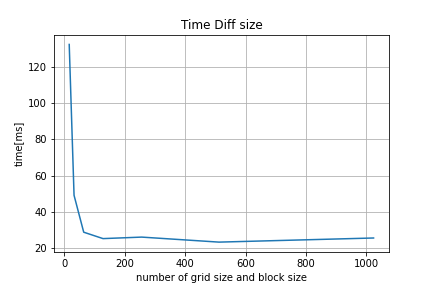
\includegraphics[width=0.80\textwidth]{Bilder/Diff_size.png}
	\caption{5 turn}
\end{figure}
There is nearly no time saving after a number of grid and block size of $64$. So the jump from $16$ to $32$ is ruffly $90$ms timesave.
\newpage
\section{Example 2 Dot Product}
\subsection{a) use two GPUs}
\begin{lstlisting}[language=C++, caption={code for a)}]
# include <stdio.h>
# include "timer.hpp"

__global__ void dot_pro_first(double *x, double *y, double *tmp, unsigned int N)
{
	unsigned int ind = threadIdx.x + blockDim.x*blockIdx.x;
	unsigned int str = blockDim.x*gridDim.x;

	__shared__ double cache[256];
	double tmpsum = 0.0;
	while(ind < N)
	{
		tmpsum += x[ind]*y[ind];
		ind += str;
	}
	cache[threadIdx.x] = tmpsum;
	__syncthreads();
	for(int i = blockDim.x/2; i>0; i/=2)
	{
			__syncthreads();
		if(threadIdx.x < i)
		{
			cache[threadIdx.x] += cache[threadIdx.x + i];
		}
	}

	if(threadIdx.x == 0)
	{
		tmp[blockIdx.x] = cache[0];
	}
}

__global__ void dot_pro_second(double *tmp, double *dot_prd)
{
	for (int i = blockDim.x/2; i > 0; i/=2)
	{
		if(threadIdx.x < i)
		{
			tmp[threadIdx.x] += tmp[threadIdx.x + i];
		}
	}
	__syncthreads();

	if(threadIdx.x == 0)
	{
		*dot_prd = tmp[0];
	}
}

int main (void)
{
	int N = 10000;
	int s = 256;
	int anz = 10;
	double *px, *py, *d_px, *d_py;
	double *prod, *d_prod, *d_tmp;
	Timer timer;

	prod = new double[N];
	px = new double[N];
	py = new double[N];
	
	for (int i = 0; i < N; i++)
	{
		px[i] = 1;
		py[i] = 3;
	}
	cudaMalloc(&d_px, N*sizeof(double));
	cudaMalloc(&d_py, N*sizeof(double));
	cudaMalloc(&d_prod, sizeof(double));
	cudaMalloc(&d_tmp, s*sizeof(double));	
	cudaMemcpy(d_px, px, N*sizeof(double), cudaMemcpyHostToDevice);
	cudaMemcpy(d_py, py, N*sizeof(double), cudaMemcpyHostToDevice);
	cudaDeviceSynchronize();
	timer.reset();
	for (int i = 0; i < anz; i++)
	{
		dot_pro_first<<<s, s>>>(d_px, d_py, d_tmp, N);
		dot_pro_second<<<1, s>>>(d_tmp, d_prod);
		cudaDeviceSynchronize();
	}
	cudaMemcpy(prod, d_prod, sizeof(double), cudaMemcpyDeviceToHost);
	
	printf("Time: %g[ms] result: %f\n", (1000*timer.get())/anz,*prod);
	
	cudaFree(d_px);
	cudaFree(d_py);
	cudaFree(d_prod);
	free(px);
	free(py);
	free(prod);
return EXIT_SUCCESS;
}
\end{lstlisting}
\subsection{b) use a GPU and the CPU}
\begin{lstlisting}[language=C++, caption={code for a)}]
# include <stdio.h>
# include "timer.hpp"
//# include <"random">

__global__ void dot_pro(double *x, double *y, double *tmp, unsigned int N)
{
	unsigned int ind = threadIdx.x + blockDim.x*blockIdx.x;
	unsigned int str = blockDim.x*gridDim.x;
	
	__shared__ double cache[256];
	
	double tmpsum = 0.0;
	while(ind < N)
	{
		tmpsum += x[ind]*y[ind];
		ind += str;
	}
	
	cache[threadIdx.x] = tmpsum;
	
	__syncthreads();
	
	for(int i = blockDim.x/2; i>0; i/=2)
	{
		__syncthreads();
		if(threadIdx.x < i)
		{
			cache[threadIdx.x] += cache[threadIdx.x + i];
		}
	}
	
	if(threadIdx.x == 0)
	{
		tmp[blockIdx.x] = cache[0];
	}
}

int main (void)
{
	int N = 10000;
	int s = 256;
	int anz = 10;
	double *px, *py, *d_px, *d_py;
	double *prod, *d_prod;
	double *tmp, *d_tmp;
	double sumdot = 0;
	Timer timer;
	
	prod = new double[N];
	px = new double[N];
	py = new double[N];
	tmp = new double[s];


	for (int i = 0; i < N; i++)
	{
		px[i] = 1;
		py[i] = 3;
	}
	cudaMalloc(&d_px, N*sizeof(double));
	cudaMalloc(&d_py, N*sizeof(double));
	cudaMalloc(&d_prod, sizeof(double));
	cudaMalloc(&d_tmp, s*sizeof(double));
	cudaMemset(d_prod, 0.0, sizeof(double));
	
	cudaMemcpy(d_px, px, N*sizeof(double), cudaMemcpyHostToDevice);
	cudaMemcpy(d_py, py, N*sizeof(double), cudaMemcpyHostToDevice);


	cudaDeviceSynchronize();
	timer.reset();
	for (int i = 0; i < anz; i++)
	{
		dot_pro<<<s, s>>>(d_px, d_py, d_tmp, N);
		cudaDeviceSynchronize();
		
		cudaMemcpy(tmp, d_tmp, s*sizeof(double), cudaMemcpyDeviceToHost);
	
		for(int j = 0; j < s; j++)
		{
			sumdot += tmp[j];
		}
	}
	printf("Time: %g[ms] result: %f\n", (1000*timer.get())/anz,sumdot/anz);
	
	cudaFree(d_px);
	cudaFree(d_py);
	cudaFree(d_prod);
	free(px);
	free(py);
	free(prod);

return EXIT_SUCCESS;
}
\end{lstlisting}
\newpage
\subsection{c) use atomicAdd}
\begin{lstlisting}[language=C++, caption={code for a)}]
# include <stdio.h>
# include "timer.hpp"
//# include <"random">

__global__ void dot_pro(double *x, double *y, double *dot, unsigned int N)
{
	unsigned int ind = threadIdx.x + blockDim.x*blockIdx.x;
	unsigned int str = blockDim.x*gridDim.x;

	__shared__ double cache[256];

	double tmpsum = 0.0;
	while(ind < N)
	{
		tmpsum += x[ind]*y[ind];
		ind += str;
	}

	cache[threadIdx.x] = tmpsum;

	__syncthreads();

	for(int i = blockDim.x/2; i>0; i/=2)
	{
		__syncthreads();
		if(threadIdx.x < i)
		{
			cache[threadIdx.x] += cache[threadIdx.x + i];
		}
	}
	
	if(threadIdx.x == 0)
	{
		atomicAdd(dot,cache[0]);
	}
}

int main (void)
{
	int N = 10;
	int s = 256;
	int anz = 10;
	double *px, *py, *d_px, *d_py;
	double *prod, *d_prod;
	
	Timer timer;
	
	prod = new double[N];
	px = new double[N];
	py = new double[N];



	for (int i = 0; i < N; i++)
	{
		px[i] = 1;
		py[i] = 3;
	}
	cudaMalloc(&d_px, N*sizeof(double));
	cudaMalloc(&d_py, N*sizeof(double));
	cudaMalloc(&d_prod, sizeof(double));
	cudaMemset(d_prod, 0.0, sizeof(double));
	
	cudaMemcpy(d_px, px, N*sizeof(double), cudaMemcpyHostToDevice);
	cudaMemcpy(d_py, py, N*sizeof(double), cudaMemcpyHostToDevice);


	cudaDeviceSynchronize();
	timer.reset();
	for (int i = 0; i < anz; i++)
	{
		dot_pro<<<s, s>>>(d_px, d_py, d_prod, N);
		cudaDeviceSynchronize();	
		cudaMemcpy(prod, d_prod, sizeof(double), cudaMemcpyDeviceToHost);
	}
	printf("Time: %g[ms] result: %f\n", (1000*timer.get())/anz,*prod/anz);
		
	cudaFree(d_px);
	cudaFree(d_py);
	cudaFree(d_prod);
	free(px);
	free(py);
	free(prod);

return EXIT_SUCCESS;
}
\end{lstlisting}
\subsection{explenarision}
\begin{figure}[H]
	\centering
	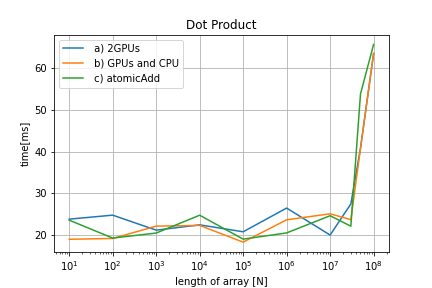
\includegraphics[width=0.80\textwidth]{Bilder/Dot_Prod.png}
	\caption{5 turn}
\end{figure}
In the end all three diferent methods needs approxematily the same amount of time. I think the third method should be the fastest method.
\end{document}